
\chapter{Literature review}\label{chap:Lit}

The following study presents an overview of the current configurations and design techniques for both operational amplifier and current-sensing circuits.
Operational amplifiers limitations are considered, as well as the system requirements. These findings are then discussed to ensure there is
enough information to aid the design process, which is followed by simulations.

\section{Operational amplifiers}\label{sec:opamps}

\subsubsection{Limitations}\label{sec:opamps_limits}
Often, it is applicable to design an amplifier using the ideal operational amplifier model, however this may be inadequate
in low voltage, high current or high frequency environments. The following are common limitations of non-ideal op-amps [1]:
\begin{itemize}
    \item Voltage supply saturation. For given k, output cannot go above $V_{ss} - k$ or below  $V_{dd} + k$.
    \item Finite bandwidth. The signal starts to cut-off at high frequencies, which can be calculated using t   he gain-bandwidth product equation.
    \item Offset voltage/bias current. Even with no input, there exists a small "offset voltage" and "bias current" into the amplifier.
          This results in unwanted voltage at the output.
    \item Finite slew rate. The output cannot change quicker than a specific rate. This is different to the high-cutoff, but has a similar limiting effect.
    \item Finite common-mode rejection ratio (CMRR). An op-amp should only amplify $V_{+} - V_{-}$, but also amplifies the unwanted common signal (e.g. noise) on both inputs.
\end{itemize}

\subsubsection{Considerations}\label{sec:opamps_considerations}
System requirements should first be considered in order to attain an overview of the specifications:
\begin{itemize}
    \item The output range of the circuit should be from 0.1 to 3 V. Since a low-side current-sense resistor will be used, this means initial measurements will be at a lower voltage initially.
    \item The step response of the circuit should reach 90\% of its output in less than 100 ms. The op-amps slew rate should be analyzed to ensure this condition is met.
    \item Noise above 1 kHz should be filtered out such that a 10 mV, 1 kHz signal at the input is less than 250 mV at the output. Filter options should therefore be researched.
\end{itemize}

It is clear that voltage supply saturation, slew rate and CMRR are the main parameters to be considered. A filter circuit should also be designed for noise specifications.

\subsubsection{MCP6242}\label{sec:opamps_MCP6242}
The op-amp used in this project is the MCP6242. Listed below are its notable parameters [2]:
\begin{itemize}
    \item Typical CMMR of 75 dB (DC) to 65 dB (1 kHz).
    \item Ability to output between 0.035 and 5.465 V if $V_{ss}$ = 6 V and $V_{dd}$ = 0 V
    \item Slew rate of 0.3 V/uS.
\end{itemize}

\subsubsection{Configurations}\label{sec:opamps_configs}
A number of well-known op-amp configurations exist that all achieve slightly different amplification goals. The following list compares common configurations [3] which may achieve this project's goal
of amplifying a small-signal voltage across a resistor. The figures below also include a modified non-inverting amplifier to allow for input signal filtering:
\begin{center}

    \begin{tabular}{|p{3.5cm}|p{6cm}|p{6cm}|}
        \hline
        Type            & Advantages                                      & Disadvantages                               \\
        \hline
        Non-inverting   & - Simple to design and build                    & - Large input bias currents                 \\
                        & - High input impedance                          & - Amplifies noise from input                \\
        \hline
        Differential    & - Good noise rejection                          & - Complex design                            \\
                        & - Flexible                                      & - Low input impedance                       \\
        \hline
        Instrumentation & - Same as differential                          & - Complex and expensive design              \\
                        & - Very high input impedance                     &                                             \\
        \hline
    \end{tabular}
\end{center}

\begin{figure}[!h]
    \centering
    \begin{minipage}{.23\textwidth}
        \centering
        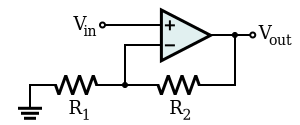
\includegraphics[width=.8\linewidth]{Figures/Op-Amp_Non-Inverting_Amplifier}
        \captionof{figure}{Non-inverting amplifier [3]}
        \label{fig:opamp-non-inverting}
    \end{minipage}
    \begin{minipage}{.23\textwidth}
        \centering
        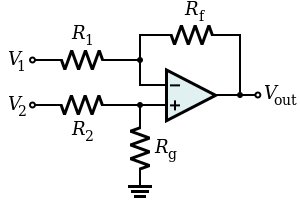
\includegraphics[width=.8\linewidth]{Figures/Op-Amp_Differential_Amplifier}
        \captionof{figure}{Differential amplifier [3]}
        \label{fig:opamp-differential}
    \end{minipage}
    \begin{minipage}{.23\textwidth}
        \centering
        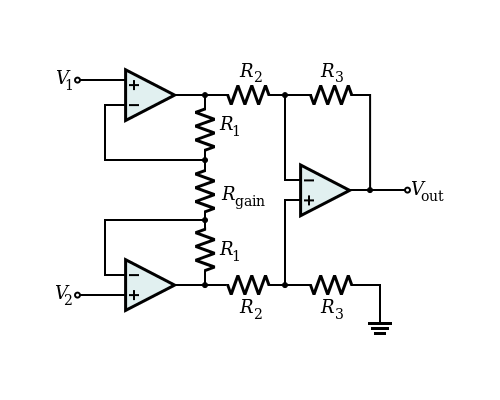
\includegraphics[width=0.9\linewidth]{Figures/Op-Amp_Instrumentation_Amplifier}
        \captionof{figure}{Instrumentation amplifier [3]}
        \label{fig:opamp-instrumentation}
    \end{minipage}
    \begin{minipage}{.23\textwidth}
        \centering
        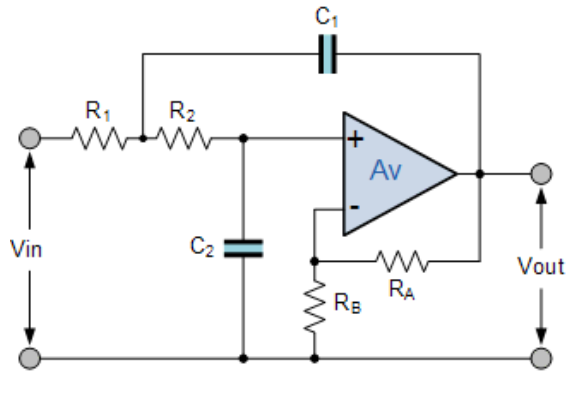
\includegraphics[width=0.8\linewidth]{Figures/Op-Amp_Non-Inverting_Filter}
        \captionof{figure}{Modified non-inverting amplifier [4]}
        \label{fig:opamp-non-inverting-filter}
    \end{minipage}    

\end{figure}

\pagebreak
\section{Current sensing}\label{sec:cursens}

\subsubsection{Sensing Techniques}\label{sec:cur_sum}
Measurement techniques are usually either "invasive" or "non-invasive". Invasive techniques tap into the circuit directly and often have a significant affect
on its operation, whereas non-invasive techniques might use e.g. the circuit's magnetic flux to determine the strength of the current.
A list of a few of these techniques [5] include:
\begin{itemize}
    \item Current-sensing resistor in series, which uses Ohm's law with a voltage measurement to calculate current.
    \item Hall element sensors, which determine the strength of current based on how much its magnetic field "bends" another current left and right, thereby creating a potential difference.
    \item Coil techniques, which make using of Faraday's law.
\end{itemize}

\begin{figure}[h!]
    \centering
    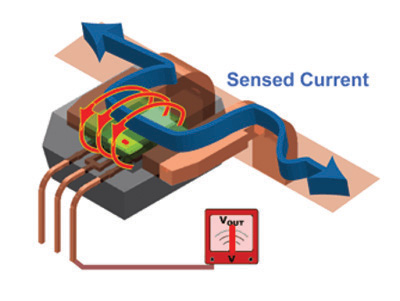
\includegraphics[width=.3\linewidth]{Figures/hall-effect-cs}    
    \captionof{figure}{Illustration of Hall Effect Sensors}
    \label{fig:hall-effect}
  \end{figure}

\subsubsection{High-side vs low-side sensing}\label{sec:cur_highlow}
These two techniques refer to the placement of a current-sense resistor relative to the load. For circuits which draw higher currents, high-side sensing can be used
(placing the resistor closer to the positive of the voltage source) and is often more convenient. Low-side sensing, on the other hand, can potentially cause ground loop
issues [6]. Low-side sending, however, also has the ability to detect faults earlier.

\subsubsection{AC, DC, and Power Requirements}\label{sec:cur_acdc}
As mentioned earlier, there are various non-invasive and even wireless techniques to measure current. Faraday's law is used to do measurements using induction, whereas
the Hall effect and sense resistors are often used in the DC case. The wireless techniques have benefits over resistors, which often have to have
relatively high power handling capabilities as they are configured to pass through the current drawn by the actual load.
